%%%%%%%%%%%%%%%%%%%%%%%%%%%%%%%%%%%%%%%%%
% Short Sectioned Assignment
% LaTeX Template
% Version 1.0 (5/5/12)
%
% This template has been downloaded from:
% http://www.LaTeXTemplates.com
%
% Original author:
% Frits Wenneker (http://www.howtotex.com)
%
% License:
% CC BY-NC-SA 3.0 (http://creativecommons.org/licenses/by-nc-sa/3.0/)
%
%%%%%%%%%%%%%%%%%%%%%%%%%%%%%%%%%%%%%%%%%

%----------------------------------------------------------------------------------------
%	PACKAGES AND OTHER DOCUMENT CONFIGURATIONS
%----------------------------------------------------------------------------------------

\documentclass[paper=a4, fontsize=11pt]{scrartcl} % A4 paper and 11pt font size

\usepackage[T1]{fontenc} % Use 8-bit encoding that has 256 glyphs
\usepackage{fourier} % Use the Adobe Utopia font for the document - comment this line to return to the LaTeX default
\usepackage[english]{babel} % English language/hyphenation
\usepackage{amsmath,amsfonts,amsthm} % Math packages
\usepackage{graphicx}


\usepackage{lipsum} % Used for inserting dummy 'Lorem ipsum' text into the template

\usepackage{sectsty} % Allows customizing section commands
\allsectionsfont{\centering \normalfont\scshape} % Make all sections centered, the default font and small caps

\usepackage{fancyhdr} % Custom headers and footers
\pagestyle{fancyplain} % Makes all pages in the document conform to the custom headers and footers
\fancyhead{} % No page header - if you want one, create it in the same way as the footers below
\fancyfoot[L]{} % Empty left footer
\fancyfoot[C]{} % Empty center footer
\fancyfoot[R]{\thepage} % Page numbering for right footer
\renewcommand{\headrulewidth}{0pt} % Remove header underlines
\renewcommand{\footrulewidth}{0pt} % Remove footer underlines
\setlength{\headheight}{13.6pt} % Customize the height of the header

\numberwithin{equation}{section} % Number equations within sections (i.e. 1.1, 1.2, 2.1, 2.2 instead of 1, 2, 3, 4)
\numberwithin{figure}{section} % Number figures within sections (i.e. 1.1, 1.2, 2.1, 2.2 instead of 1, 2, 3, 4)
\numberwithin{table}{section} % Number tables within sections (i.e. 1.1, 1.2, 2.1, 2.2 instead of 1, 2, 3, 4)

\setlength\parindent{0pt} % Removes all indentation from paragraphs - comment this line for an assignment with lots of text

%----------------------------------------------------------------------------------------
%	TITLE SECTION
%----------------------------------------------------------------------------------------

\newcommand{\horrule}[1]{\rule{\linewidth}{#1}} % Create horizontal rule command with 1 argument of height

\title{	
\normalfont \normalsize 
\textsc{North Carolina State University} \\ [25pt] % Your university, school and/or department name(s)
\horrule{0.5pt} \\[0.4cm] % Thin top horizontal rule
\huge Homework 1 for Chapter 2 \\ % The assignment title
\horrule{2pt} \\[0.5cm] % Thick bottom horizontal rule
}

\author{Jinwen Zhao, Chang Liu, Ling Zhang} % Your name

\date{\normalsize\today} % Today's date or a custom date

\begin{document}

\maketitle % Print the title

%----------------------------------------------------------------------------------------
%	PROBLEM 1
%----------------------------------------------------------------------------------------

\section*{Problem 1}
\paragraph{\textbf{Problem 2 Page 119 Part a}} Let $ g(t) $ be the approximation to $ f $,
\begin{align*}
	\|f-g\|_{\infty}&=\sup_{1\leq i\leq N} | f(t)-g(t)|\\
	g(t)&=c=\dfrac{y+1}{2}
\end{align*}

Therefore, $ \|f-g\|_{\infty}=\dfrac{y-1}{2} $.

\paragraph{\textbf{Problem 2 Page 119 Part b}} Let $ g(t) $ be the approximation to $ f $,
\begin{align*}
	\|f-g\|_2&=({\sum_{i=1}^{N}|f(t_i)-g(t_i)|^{2}} )^{\frac{1}{2}}\\
			&=\sqrt{(N-1)(c-1)^2+(c-y)^2} = \sqrt{Nc^2-2(N-1+y)c+(N-1)+y^2}
\end{align*}\\
Solve this the function $ h(c)=Nc^2-2(N-1+y)c+(N-1)+y^2 $ for the minimum value and we get $ c=\dfrac{N-1+y}{N} $. Therefore $ \|f-g\|_2=y^2(1-\dfrac{1}{N})-y(\dfrac{2N-2}{N})+\dfrac{N-1}{N} $

\paragraph{\textbf{Problem 2 Page 119 Part c}} As $ N\rightarrow \infty $, the constant in the least square approximation goes to 1. It shows the least square approximation weights less on the outliers than the infinity approximation. Request more input.

\newpage
\paragraph{\textbf{Problem 5 Page 119 Part a}}  
Define the following $ \hat{f}(x)=1+cx $ and $ f(x)=e^x $.\\
\begin{align*}
	\|\hat{f}-f\|^2_2=&\int_{0}^{1}|e^x-1-cx|^2 dx=\int_{0}^{1}e^{2x}-2e^x(1+cx)+(1-cx)^2dx\\
	=&\int_{0}^{1}e^{2x}-(2e^x+2ce^xx)+(1-2cx+c^2x^2)dx\\
	=&\dfrac{1}{3}c^2-c+C
\end{align*}
$ C $ is some constant that we do not care. Minimize the function $ h(c)=\dfrac{1}{3}c^2-c+C $ and the minimum reaches at $ c=\dfrac{3}{2} $.

\paragraph{\textbf{Problem 5 Page 119 Part b}}  
Solve for the general case, $ max_{0 \leq x\leq 1} |e^x-(1+cx)| $. Let $  f_c(x)=e^x-(1+cx) $ and,
\begin{align*}
	f_c^\prime (x)&=e^x-c
\end{align*}
$ c=1 $. $ f_1(x) $ is monotonic increasing in the interval $ [0,1] $ and the minimum is $ f_1(0)=0$. Then $ |e_1(x)|=f_1(x) $. The maximum is at $ x=1 $ and the max error is $ e-2 $. For the case $ c=\dfrac{3}{2} $, $ f_{\frac{3}{2}}(x)$ is decreasing at $ [0,ln \frac{3}{2}] $ and increasing at $ [ln \frac{3}{2},1] $. The minimum is $ f_{\frac{3}{2}}(ln\frac{3}{2})<0 $. Therefore $ \max e_2(x)=|f_{\frac{3}{2}}(x)| $ is either reached at the endpoint, $ \{0, 1\} $, or at $ x=\ln \frac{3}{2} $. Plug in and the maximum of $ e_2(x) $ at the interval $ [0,1] $ is $ e-2.5  $ at the endpoint $ x=1 $.

\paragraph{\textbf{Problem 5 Page 119 Part c}} 
Define the following minimization problem,
\begin{align*}
	\min_{0\leq x\leq 1} \|e^x-(1+c_1x+c_2x^2) \|_2^2
\end{align*} 
\begin{align*}
	\int_{0}^{1}(e^x-(1+c_1x+c_2x^2))^2dx&=\frac{1}{3}c_1^2+\frac{1}{2}(c_2-2)c_1+\frac{1}{5}c_2^2+C=g(c_1,c_2)
\end{align*}
\begin{align*}
	\dfrac{\partial g}{\partial c_1}&=\dfrac{1}{2}(c_2-2)+\dfrac{2}{3}c_1=0\\
	\dfrac{\partial g}{\partial c_2}&=\dfrac{1}{2}c_1+\dfrac{2}{5}c_2+\dfrac{14}{3}-2e=0\\
\end{align*}
Solve this system of equations and get $ c_1=0.9031 $ and $ c_2=0.7959 $.

\begin{figure}[h]
\centering
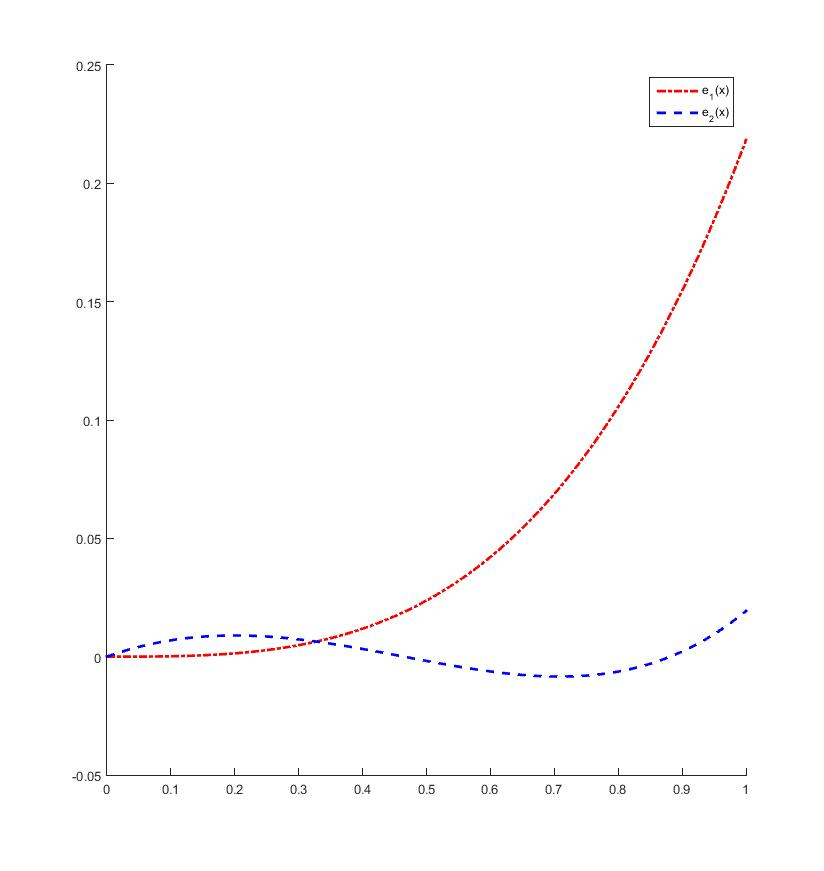
\includegraphics[width=0.5\linewidth]{../Q5}
\caption{Error curves of $ e_1(x) $ and $ e_2(x) $}
\label{fig:Q5}
\end{figure}

\newpage
\paragraph{\textbf{Problem 33 Page 126}} 
We use two different method to solve this problem.
\begin{enumerate}
	\item Lagrange Interpolation\\
		\begin{align*}
			i&=0,~l_0(x)=\dfrac{x-x_1}{x_0-x_1}\dfrac{x-x_2}{x_0-x_2}\\
			i&=1,~l_0(x)=\dfrac{x-x_0}{x_1-x_0}\dfrac{x-x_2}{x_1-x_2}\\
			i&=2,~l_0(x)=\dfrac{x-x_0}{x_2-x_0}\dfrac{x-x_1}{x_2-x_1}\\
			p(x)&=\ln(10)*l_0(x)	+ \ln(11)*l_1(x)+\ln(12)*l_2(x)
		\end{align*}
		The relative error is $ 0.10282\% $
	
	\item Newton's Interpolation\\
	Chang Chang
\end{enumerate}
\newpage

\paragraph{\textbf{Problem 36 Page 126 Part a}} 

We know that,
\begin{align*}
	|E(x)| = &|e^x-p_n(f;x)| = |\dfrac{e^{\xi(x)}}{(n+1)!}\prod_{i=0}^{n}(x-x_i)|\\
		 = &\dfrac{e^{\xi(x)}}{(n+1)!}\prod_{i=0}^{n}|(x-\dfrac{i}{n})|\\
 		 = &\dfrac{e^{\xi(x)}}{(n+1)!}\prod_{i=0}^{n}\sqrt{|(x-\dfrac{i}{n})(x-\dfrac{n-i}{n})|}\\
\end{align*}
We then show the hint is true by a simple maximization problem, $ \forall i=0\cdots n $
\begin{align*}
	\max_{0\leq x\leq 1} |(x-\dfrac{i}{n})(x-\dfrac{n-i}{n})|	
\end{align*}
Define $ f(x)=(x-\dfrac{i}{n})(x-\dfrac{n-i}{n}) $ and the minimum point is achieved at $ x=\frac{1}{2} $. That is, $ |f(x)| $ achieves maximum of $ max = |(\frac{1}{2}-\dfrac{i}{n})(\frac{1}{2}-\dfrac{n-i}{n})|\leq |(\frac{1}{2}-0)(\frac{1}{2}-1)|=\frac{1}{4} $ at $ x=\frac{1}{2} $.
\begin{align*}
	\max_{0\leq x\leq 1}|E(x)|\leq \dfrac{e^{1}}{(n+1)!}\dfrac{1}{2^n}
\end{align*}
Solve the following inequality,
\begin{align*}
	\dfrac{e^{1}}{(n+1)!}\dfrac{1}{2^n}\leq 10^{-6}
\end{align*}
The smallest n is 9.
\paragraph{\textbf{Problem 36 Page 126 Part b}} 
What is connection between the Talyor polynomial and the interpolation polynomial???
\newpage

\paragraph{\textbf{Problem 46 Page 128}} 
We know that,
\begin{align*}
	T_n(\cos\theta)=\cos(n\theta)
\end{align*}
Take derivative with respect to $ \theta $ and set it to $ \dfrac{\pi}{2} $,
\begin{align*}
	T_n^\prime(\cos\theta)&=n\sin(n\theta)\sin(\theta)\\
	T_n^\prime(0)&=n\sin(\dfrac{n\pi}{2})
\end{align*}




\newpage
\section*{Programming Assignment}
\paragraph{Problem 9 Page 137}

\section{Problem title}

\lipsum[2] % Dummy text

\begin{align} 
\begin{split}
(x+y)^3 	&= (x+y)^2(x+y)\\
&=(x^2+2xy+y^2)(x+y)\\
&=(x^3+2x^2y+xy^2) + (x^2y+2xy^2+y^3)\\
&=x^3+3x^2y+3xy^2+y^3
\end{split}					
\end{align}

Phasellus viverra nulla ut metus varius laoreet. Quisque rutrum. Aenean imperdiet. Etiam ultricies nisi vel augue. Curabitur ullamcorper ultricies

%------------------------------------------------

\subsection{Heading on level 2 (subsection)}

Lorem ipsum dolor sit amet, consectetuer adipiscing elit. 
\begin{align}
A = 
\begin{bmatrix}
A_{11} & A_{21} \\
A_{21} & A_{22}
\end{bmatrix}
\end{align}
Aenean commodo ligula eget dolor. Aenean massa. Cum sociis natoque penatibus et magnis dis parturient montes, nascetur ridiculus mus. Donec quam felis, ultricies nec, pellentesque eu, pretium quis, sem.

%------------------------------------------------

\subsubsection{Heading on level 3 (subsubsection)}

\lipsum[3] % Dummy text

\paragraph{Heading on level 4 (paragraph)}

\lipsum[6] % Dummy text

%----------------------------------------------------------------------------------------
%	PROBLEM 2
%----------------------------------------------------------------------------------------

\section{Lists}

%------------------------------------------------

\subsection{Example of list (3*itemize)}
\begin{itemize}
	\item First item in a list 
		\begin{itemize}
		\item First item in a list 
			\begin{itemize}
			\item First item in a list 
			\item Second item in a list 
			\end{itemize}
		\item Second item in a list 
		\end{itemize}
	\item Second item in a list 
\end{itemize}

%------------------------------------------------

\subsection{Example of list (enumerate)}
\begin{enumerate}
\item First item in a list 
\item Second item in a list 
\item Third item in a list
\end{enumerate}

%----------------------------------------------------------------------------------------

\end{document}